\documentclass[aspectratio=169]{beamer}
\usepackage{babel}
\usepackage{array, colortbl, tikz, transparent, listings, pgfplots}
\usepackage[export]{adjustbox}
\usepackage[skins,theorems]{tcolorbox}
\usepackage[backend=biber,style=verbose-ibid,citetracker=true,ibidtracker=constrict,autocite=footnote]{biblatex}

\setbeamercovered{transparent}
\lstdefinelanguage{Rust}{
    sensitive=true,
    morekeywords={as, break, const, continue, crate, else, enum, extern, false, fn, for, if, impl, in, let, loop, match, mod, move, mut, pub, ref, return, self, Self, static, struct, super, trait, true, type, unsafe, use, where, while, async, await, dyn, Result, Option, Ok, Err, panic},
    morecomment=[l]{//},
    morecomment=[s]{/*}{*/},
    morestring=[b]",
    morestring=[b]',
}
\lstdefinelanguage{Yaml}{
    sensitive=true,
    morekeywords={true, false, null, particles, type, cuboid, foreach, position, velocity, mass, sigma, brownian_sigma},
    morecomment=[l]{\#},
    morestring=[b]",
}
\lstset{
    language=Rust,
    basicstyle=\ttfamily\small,
    keywordstyle=\color{blue}\bfseries,
    stringstyle=\color{red},
    commentstyle=\color{teal},
    morekeywords={Result, Option, Ok, Err, Some, None, panic},
    breaklines=true
}
\usetikzlibrary{automata,positioning}
\addbibresource{Reference.bib}

\title{Rust vs C++: Brief Introduction}
\author{Anatoly Weinstein}
\date{30th of April 2025}

\newcommand{\framebackground}[3]{
    \begin{tikzpicture}
        \transparent{#1}
        \node[inner sep=0] at (current page.center) {
            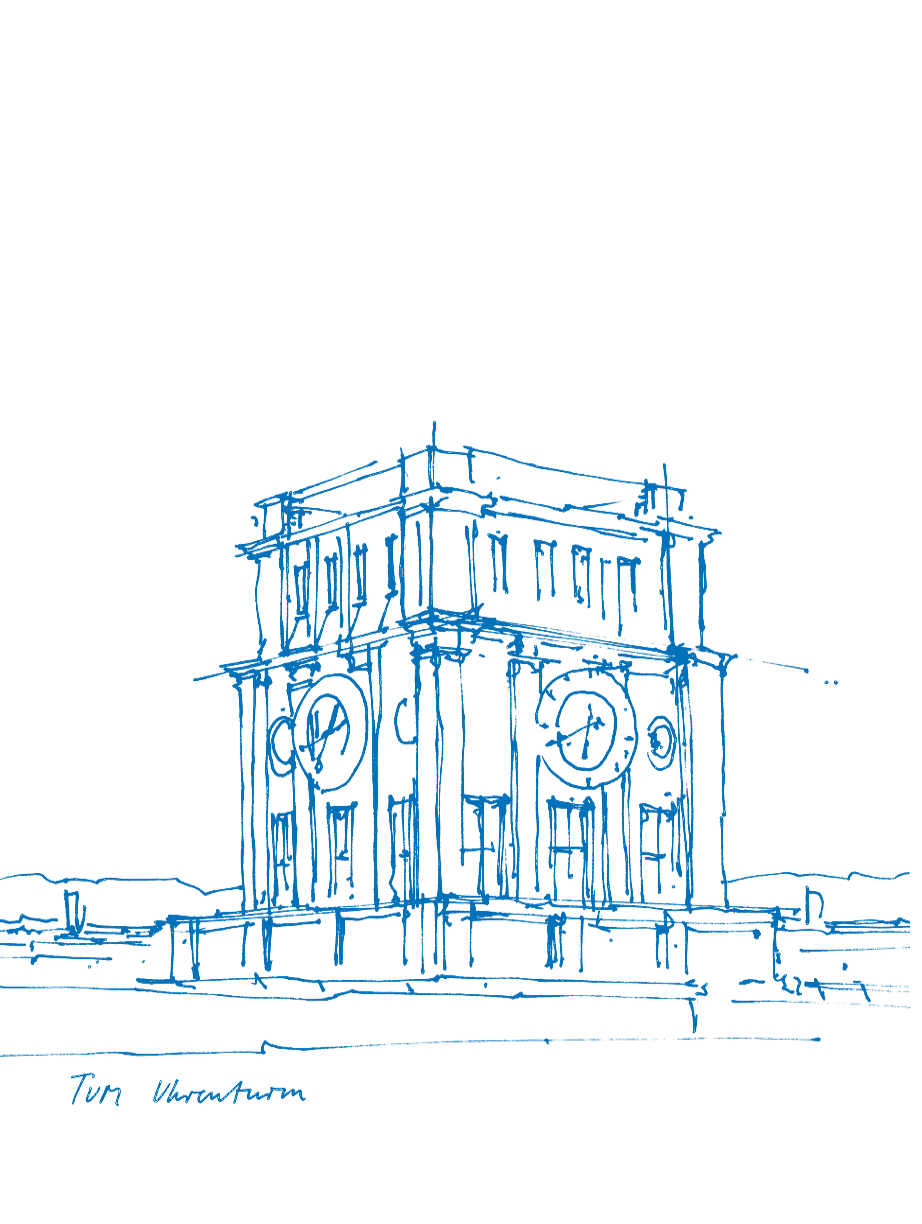
\includegraphics[height=\paperheight, right]{./media/tum-uhrenturm.png}
        };
        \transparent{#2}
        \node[anchor=south, text width=\paperwidth, text height=1.5cm, draw=none, align=center] at (current page.south) {
            \insertpagenumber
        };
        \transparent{#3}
        \node[anchor=south, text width=\paperwidth, text height=1.5cm, draw=none, align=right] at (current page.south) {
            \small Anatoly W. \,\,
        };
    \end{tikzpicture}
}

\newcommand{\headerframe}{
    \usebackgroundtemplate{
        \framebackground{0.2}{1}{1}
    }
}

\newcommand{\simpleframe}{
    \usebackgroundtemplate{
        \framebackground{0}{1}{1}
    }
}

\newcommand{\nofooterframe}{
    \usebackgroundtemplate{
        \framebackground{0}{0}{1}
    }
}

\newcommand{\blue}[1]{{\color{beamer@blendedblue} #1}}
\newcommand{\yellow}[1]{{\color[HTML]{AF8F10} #1}}
\newcommand{\gray}[1]{{\color[HTML]{8F8F8F} #1}}
\newcommand{\red}[1]{{\color[HTML]{FF5F5F} #1}}

\begin{document}

%
% Frame
%
\usebackgroundtemplate{\framebackground{0.2}{0}{0}}
\begin{frame}
    \maketitle
\end{frame}

\nofooterframe\begin{frame}[t, fragile]{First of all: I was wrong! (kind of)}
    So far: Assumption that Rust does overflow checks that is why the code is slower.

    \vspace{1em}
    \red{Wrong!}

    \vspace{1em}
    While it is correct to say, that when you start cargo in development with `\texttt{cargo run}' overflows will panic, the release build is compiled without overflow checks.\footcite{rust-profiles}

    \begin{lstlisting}
[profile.dev]
opt-level = 0
debug = true
overflow-checks = true

[profile.release]
opt-level = 3
debug = false
overflow-checks = false
    \end{lstlisting}
\end{frame}

\nofooterframe\begin{frame}[t, fragile]{First of all: I was wrong! (kind of)}
    However this only affects arithmetic overflows. Out of bounds checks on arrays, slices and vectors are still present in release build and explain the slowdown in the `for each pair' loop.
\end{frame}

\nofooterframe\begin{frame}[t, fragile]{Another awkward observation: Compilation Flags Magic\footcite{benchmark-32}}
    I added more compilation flags to Rust and this changes the results significantly.

    \vspace{0.5em}
    \begin{center}
        \begin{tikzpicture}
            \begin{axis}[
                width=\textwidth,  
                height=0.7\textheight,
                xlabel={},
                ylabel={Runtime (ms)},
                xtick={0, 20, 50},
                scaled x ticks=false,  
                scaled y ticks=false,
                ymajorgrids=true, 
                grid style=dashed,
                xmin=-5,
                xmax=55,
                legend style={at={(0.05,0.95)},anchor=north west},
            ]

            \addplot[
                color=blue,
                mark=square,
                line width=1pt,
                ]
                coordinates {
                    (0, 122)(20, 862)(50, 1979)
                };

            \addplot[
                color=gray!50,
                mark=square,
                line width=1pt,
                ]
                coordinates {
                    (0, 112)(20, 615)(50, 1372)
                };

            \addplot[
                color=orange,
                mark=triangle,
                line width=1pt,
                ]
                coordinates {
                    (0, 33)(20, 383)(50, 909)
                };

            \addplot[
                color=cyan,
                mark=square,
                line width=1pt,
                ]
                coordinates {
                    (0, 88)(20, 159)(50, 269)
                };

            \addplot[
                color=red,
                mark=triangle,
                line width=1pt,
                ]
                coordinates {
                    (0, 17)(20, 50)(50, 101)
                };

            \legend{C++ (Sum), C++ (Sum Parallel), Rust (Sum), C++ (Linked Cells), Rust (Linked Cells)}
            \end{axis}
        \end{tikzpicture}
    \end{center}

    \blue{Note:} C++ performs worse in this benchmark. My guess is that OMP introduced general overhead in the binary and maybe the outlining does not work correctly. 
    
    % I don't know core count and threads for Github Actions runners. On my PC the parallel direct sum is a lot faster (193ms for 50 steps, versus 1199ms for single-threaded, outperformed by 158ms for C++ Linked Cells).
\end{frame}

\nofooterframe\begin{frame}[t]{Tuned Benchmarks \footcite{benchmark-22} \footcite{benchmark-32}}
    Here is the "best of" comparison, using \texttt{benchmark-32} for Rust and \texttt{benchmark-22} for C++:

    \vspace{0.5em}
    \begin{center}
        \begin{tikzpicture}
            \begin{axis}[
                width=\textwidth,  
                height=0.7\textheight,
                xlabel={},
                ylabel={Runtime (ms)},
                xtick={0, 20, 50},
                scaled x ticks=false,  
                scaled y ticks=false,
                ymajorgrids=true, 
                grid style=dashed,
                xmin=-5,
                xmax=55,
                legend style={at={(0.05,0.95)},anchor=north west},
            ]

            \addplot[
                color=blue,
                mark=square,
                line width=1pt,
                ]
                coordinates {
                    (0, 109)(20, 509)(50, 1080)
                };

            \addplot[
                color=orange,
                mark=triangle,
                line width=1pt,
                ]
                coordinates {
                    (0, 33)(20, 383)(50, 909)
                };

            \addplot[
                color=cyan,
                mark=square,
                line width=1pt,
                ]
                coordinates {
                    (20, 83)(50, 178)
                };

            \addplot[
                color=red,
                mark=triangle,
                line width=1pt,
                ]
                coordinates {
                    (0, 17)(20, 50)(50, 101)
                };

            \legend{C++ (Sum), Rust (Sum), C++ (Linked Cells), Rust (Linked Cells)}
            \end{axis}
        \end{tikzpicture}
    \end{center}
\end{frame}

\nofooterframe\begin{frame}[t]{Benchmark: Outlining}
    Done with new macro keyword \texttt{outline}, which we set conditionally to prevent inlining. The idea is to preserve the debug symbols in the stack similarly for Rust and C++.

    \red{TBA: I have not finished this SORRY!}
\end{frame}

\nofooterframe\begin{frame}[t]{Change of Opinion}
    After all the optimizations, selectively using best benchmark results and playing with compiler flags I have arrived at the following wisdoms:

    \begin{itemize}
        \item C++ and Rust can wield comparable performance, Rust even outperforming C++ in today's benchmarks.
        \item You shall not judge a languages' performance based on the first benchmark I ran, especially if I have no clue.
    \end{itemize}

    \begin{columns}
        \begin{column}{0.4\textwidth}
            \centering
            
\includegraphics[width=0.8\textwidth]{./media/meme-farmer.png}
        \end{column}
        \begin{column}{0.6\textwidth}
            \centering
            
\includegraphics[width=\textwidth]{./media/meme-this-is-fine.png}
        \end{column}
    \end{columns}
\end{frame}

% \nofooterframe\begin{frame}[t]{Benchmark: Outlining}
%     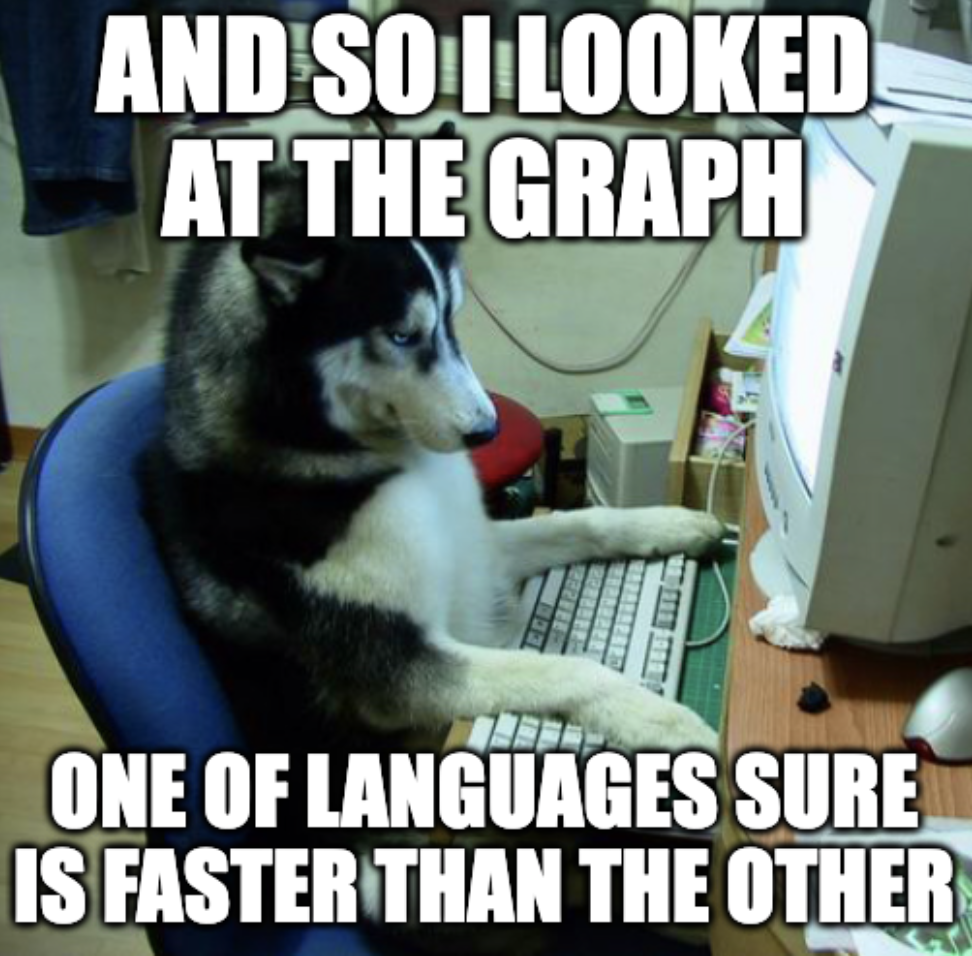
\includegraphics[width=\textwidth]{./media/meme-no-idea.png}
% \end{frame}

\headerframe\begin{frame}[allowframebreaks]{References}
  \printbibliography
\end{frame}

\end{document}
